\documentclass[letterpaper, reqno,11pt]{article}
\usepackage[margin=1.0in]{geometry}
\usepackage{color,latexsym,amsmath,amssymb,graphicx,float,listings,tikz}
\usepackage{hyperref}

\hypersetup{
colorlinks=true,
linkcolor=magenta,
filecolor=magenta,
urlcolor=cyan,
}

\lstset{
  basicstyle=\ttfamily,
  columns=fullflexible,
  frame=single,
  breaklines=true,
  postbreak=\mbox{\textcolor{red}{$\hookrightarrow$}\space},
}

\graphicspath{ {images/} }

\begin{document}
\pagenumbering{arabic}
\title{Math 406 Homework 7}
\date{01/12/23}
\author{Xander Naumenko}
\maketitle

{\medskip\noindent\bf Question 1.} See figure \ref{fig:q1a} for the plot of the numerical solution compared to the exact, and figure \ref{fig:q1b} for the errors. Finally, see plot \ref{fig:q1c} for the plot along $-a<x<0,y=0$. One thing I noticed while solving this is that the choice of parameterization is extremely fiddly; I myself tried two and they gave fairly different solutions, and I compared to another classmate and using a third different parameterization they got a different graph as well. Given the question doesn't specify any choice of parameterization I went with my original somewhat arbitrary choice of starting at the center and proceeding counter-clockwise, but I suspect the resulting graphs vary significantly even for small choice differences.

As for the code, there were three changes. First, the parameterization for the half circle was added. Second, instead of just assigning $u$ and then directly solving for $p$ as in the original code, we follow the same procedure as in the notes to solve for $u$ and $p$ by separating them into their known and unknown quantities. Finally, the exact solution and plotting was changed to match our requirements. Here is the modified code in Laplace.m:

\begin{figure}[htpb]
    \centering
    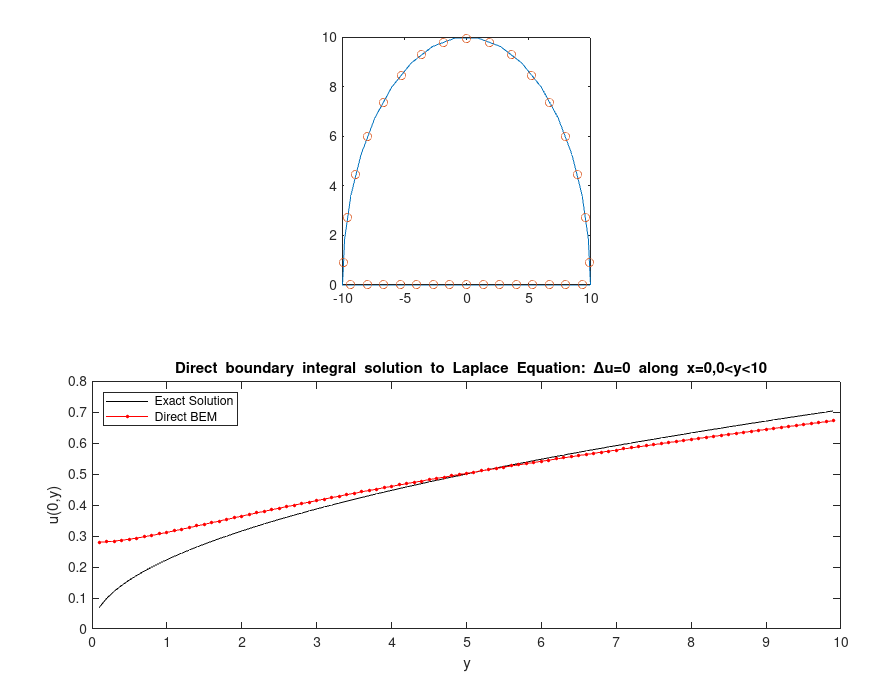
\includegraphics[width=0.8\textwidth]{q1a}
    \caption{Plot along the axis $x=0,0.1<y<9.9$.}
    \label{fig:q1a}
\end{figure}

\begin{figure}[htpb]
   \centering
   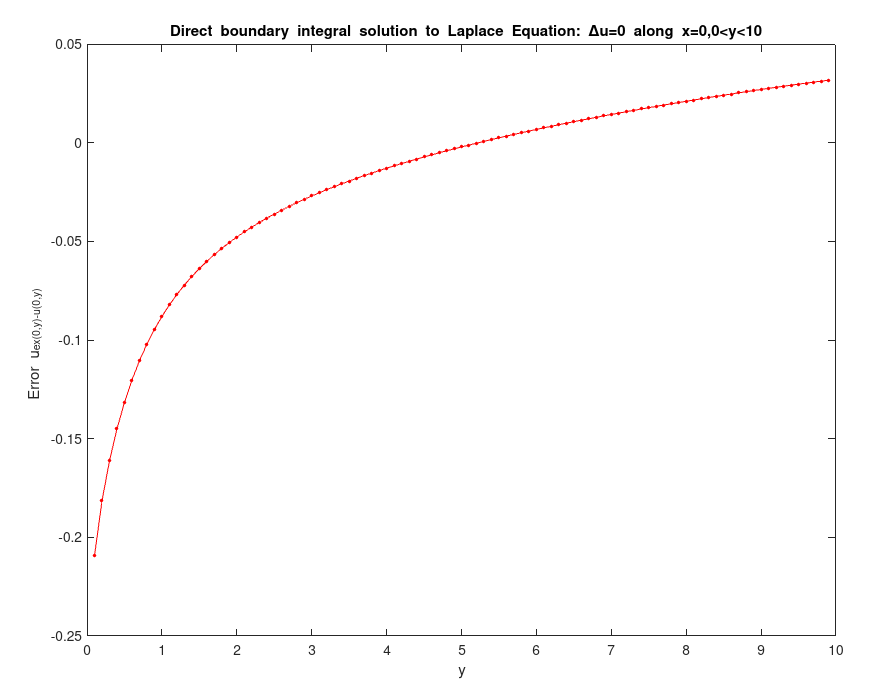
\includegraphics[width=0.8\textwidth]{q1b}
   \caption{Plot of error for figure \ref{fig:q1a}.}
   \label{fig:q1b}
\end{figure}

\begin{figure}[htpb]
   \centering
   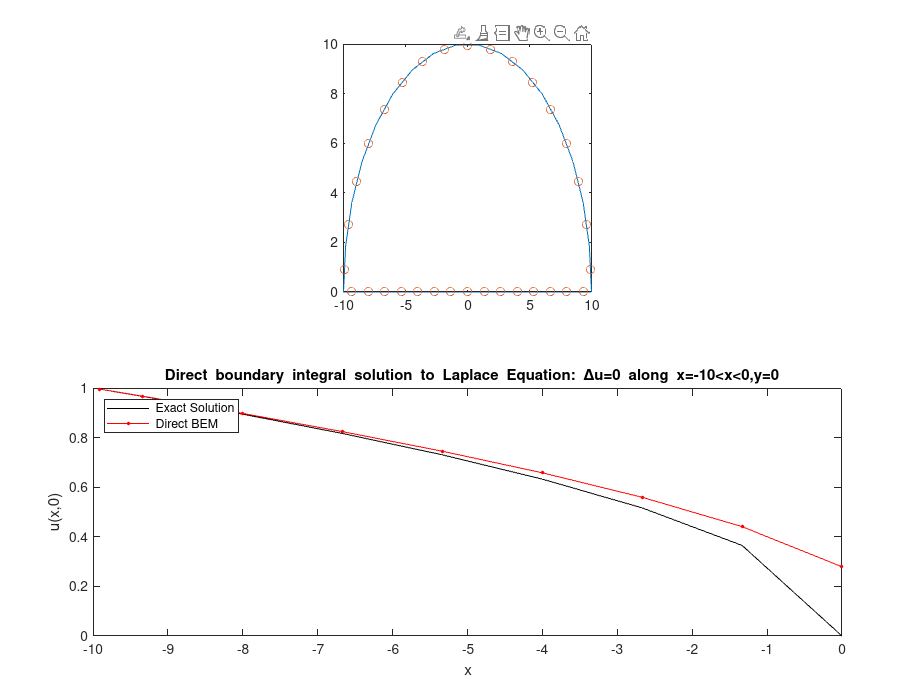
\includegraphics[width=0.8\textwidth]{q1c}
   \caption{Plot of solution along axis $-a<x<0,y=0$.}
   \label{fig:q1c}
\end{figure}

\begin{lstlisting}
clear;clf;
% Direct BEM solution to Laplaces equation on a circle of radius R
% nabla^2 u = 0 0<=r<R -pi<theta<pi
% with Dirichlet BC u(R,theta) = [ 1 for 0<theta<pi
%                                [ 0 for -pi<theta<0
%
% define elements on the boundary of a circle
N=32;   % Number of line segments
R=10;   % radius of circle
Ns=1:N;

% % Old parameterization, pretty sure it's valid but seems to give worse
% % result for some reason
dth=pi/(N/2+1);
th=dth:dth:pi-dth;
% define beginning points of the line segments
xb=R*cos(th);  
yb=R*sin(th);
dx = 2*R/(N/2-1);
xb = [dx/2:dx:R, xb, -R:dx:dx/2];
yb = [zeros(1,N/4), yb, zeros(1,N/4+1)];

% dth = pi/(N/2);
% th = 0:dth:pi;

% dx = 2*R / (N/2-1);

% xb = [0:dx:R,R*cos(th),-R:dx:0];
% yb = [zeros(1,N/4),R*sin(th),zeros(1,N/4)];

xe=xb*0;ye=yb*0;
xe(1:N-1)=xb(2:N);xe(N)=xb(1);
ye(1:N-1)=yb(2:N);ye(N)=yb(1);
% define midpoints of the line segments
xm=0.5*(xb+xe);
ym=0.5*(yb+ye);
% determine element attributes
ah=0.5*sqrt((xe-xb).^2+(ye-yb).^2);        % half length of element
% determine tangent vectors to elements
calf=0.5*(xe-xb)./ah;                      
salf=0.5*(ye-yb)./ah; 
%generate influence matrices
for i=1:N % sending element
   % global coordinate of current sending element
   xs=xm(i);   
   ys=ym(i);
   % orientation of sending element
   ci=calf(i);
   si=salf(i);
   % half length of sending element
   as=ah(i);
   for j=1:N % receiving element
      % determine relative distance from sending element to receiving element
      x=xm(j)-xs;
      y=ym(j)-ys;
      % rotate to local sending element coordinates
      xp=x*ci+y*si;
      yp=-x*si+y*ci;
      % determine influence matrices
      G(j,i)=V(xp,yp,as);
      H(j,i)=VN(xp,yp,as);
   end
end

% set up boundary values of u/q
% Technique is taken from the notes, lecture 31
g = [zeros(1,N/4), sin(th./2)];
h = zeros(1, N/4);

A = [G(:, 1:3*N/4), -H(:,3*N/4+1:end)];
B = [H(:,1:3*N/4), -G(:,3*N/4+1:end)];

t = (A\(B*[g, h]'))';

u = [g, t(3*N/4+1:end)];
p = [t(1:3*N/4), h];

% evaluate the solution at benchmarks
ybm = 0.1:0.1:R-0.1;
xbm = 0*ybm;
ubm = 0*xbm;
for i=1:N % sending element
   % global coordinate of current sending element
   xs=xm(i);   
   ys=ym(i);
   % orientation of sending element
   ci=calf(i);
   si=salf(i);
   % half length of sending element
   as=ah(i);
   for j=1:length(ybm)
      % determine relative distance from sending element to receiving benchmark point
      x=xbm(j)-xs;
      y=ybm(j)-ys;
      % rotate to  local sending element coordinates
      xp = x*ci+y*si;
      yp =-x*si+y*ci;
      % accumulate the contributions to the potential at the bechmark point of the current sending element
      ubm(j) = ubm(j)+VN(xp,yp,as)*u(i)-V(xp,yp,as)*p(i);
   end
end
% Determine the exact solution at the benchmarks
rbm = sqrt(xbm.*xbm+ybm.*ybm);thbm=atan2(ybm,xbm);
ue = sqrt(rbm./R).*sin(thbm./2);
%ue  = 0.5+atan2(2*R*rbm.*sin(thbm),R^2-rbm.^2)/pi;
% Plot solutions 
figure(1);
subplot(2,1,1),plot(xb,yb,xm(Ns),ym(Ns),'o');
axis square
subplot(2,1,2),plot(ybm,ue,'k-',ybm,ubm,'r-o','markersize',2,'markerfacecolor','r')
xlabel('y')
ylabel('u(0,y)')
legend(' Exact Solution ',' Direct BEM ','Location','NorthWest')
title(' Direct boundary integral solution to Laplace Equation: \Deltau=0 along x=0,0<y<10')
figure(2),plot(ybm,ue-ubm,'r-o','markersize',2,'markerfacecolor','r')
xlabel('y')
ylabel('Error u_ex(0,y)-u(0,y) ')
title(' Direct boundary integral solution to Laplace Equation: \Deltau=0 along x=0,0<y<10')


% evaluate the solution at benchmarks
xbm = xm(N-8:N);
ybm = 0*xbm;
ubm = 0*xbm;
rbm = sqrt(xbm.*xbm+ybm.*ybm);thbm=0*xbm+pi;
ue = sqrt(rbm./R).*sin(thbm./2);
% Plot solutions 
figure(3);
subplot(2,1,1),plot(xb,yb,xm(Ns),ym(Ns),'o');
axis square
subplot(2,1,2),plot(xbm,ue,'k-',xbm,u(N-8:end),'r-o','markersize',2,'markerfacecolor','r')
xlabel('x')
ylabel('u(x,0)')
legend(' Exact Solution ',' Direct BEM ','Location','NorthWest')
title(' Direct boundary integral solution to Laplace Equation: \Deltau=0 along x=-10<x<0,y=0')

\end{lstlisting}


\end{document}
